% !TEX TS?program = pdflatexmk
\documentclass[a4paper, 12pt]{article}
\usepackage[english]{babel}
\usepackage[utf8]{inputenc}
\usepackage[utf8]{inputenc}
% \renewcommand{\baselinestretch}{1.0} 
%MARGINS
\usepackage[left=25.4mm, right = 25.4mm, top=25.4mm, bottom=25.4mm, includefoot]{geometry}
% \geometry{a4paper, total={170mm,257mm}, left=25.4mm, right = 25.4mm, top=25.4mm, bottom=25.4mm}
\setlength{\parindent}{0in}
\usepackage{enumitem}
%Adding pictures
\usepackage{graphicx}
\usepackage{float}
%Header and footers
\usepackage{fancyhdr}
\pagestyle{fancy}
% \fancyhead{}
\fancyfoot{}
\fancyfoot[R]{ \thepage\ }
\renewcommand{\headrulewidth}{0pt} %change the pt width to insert header line
\renewcommand{\footrulewidth}{0pt} %change the pt width to insert footer line
\usepackage{amsmath}
\fancyhf{}
% \rhead{\leftmark}
% \lhead{Guides and tutorials}
\rfoot{Centre for Civil Society \hspace{1mm} \textbar \hspace{1mm} www.ccs.in \hspace{2mm} \thepage}
% \lfoot{ \leftmark } % get the section heading on the footer 
%Tables
\usepackage{booktabs}
\usepackage{subfig}
\captionsetup{aboveskip=14pt,}
%Coloured Boxes
\usepackage{xcolor}
\usepackage{mdframed}
%Custom Spacing
\usepackage{setspace}
%Defining Colours
\definecolor{CCSbrown}{RGB}{163, 86, 37}
\definecolor{CCSgrey}{RGB}{167, 169, 172}
\definecolor{CCSblack}{RGB}{64, 64, 65} 
%Heading colours 
\usepackage{sectsty}
\usepackage{titlesec}
\chapterfont{\color{blue}} % sets colour of chapters font
\sectionfont{\color{CCSbrown}} %sets colour of section font
\subsectionfont{\color{CCSblack}} %sets colour of subsection font
\subsubsectionfont{\color{CCSgrey}} %sets colour of subsubsection font
%Bibliography
\usepackage[authordate, backend=biber]{biblatex-chicago}
\addbibresource{meat.bib}
\begin{document}
%================================================== 
%TITLE PAGE
\begin{titlepage}
\begin{center}
\line(1,0){300}\\
[0.25in]
\huge{\bfseries \textcolor{CCSbrown} {Pound of Flesh: }} \\
[0.5cm]
\large {Ease of Doing Business for Slaughterhouses and Meat Shops in Delhi} \\
\line(1,0){200}\\
[1in]
\textsc{\huge Shruti Gupta, \\ Sanjari Kalantri, Shivank Singh} \\
[1.5cm]
{\Large September 2018} \\
[2.0cm]
% {\huge Researching Reality Internship 2018} \\
% [0.5cm]
{\LARGE Centre for Civil Society} \\
[0.1mm]
{\Large New Delhi, India} \\
[2.0cm]
%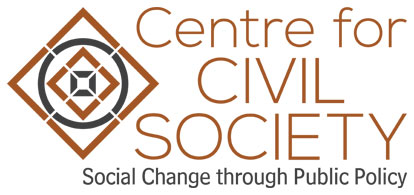
\includegraphics[width = 75mm]{C:/Users/Dell/Desktop/CCS/TEX/New Folder/CCSlogo.jpg}
\end{center}
\end{titlepage}
%=====================TOC=============================================== 
\tableofcontents
%======================LIST OF ABBREVIATIONS================================ 
\newpage
\newlist{abbrv}{itemize}{1}
\setlist[abbrv,1]{label=,labelwidth=1in,align=parleft,itemsep=0.1\baselineskip,leftmargin=!}
\section*{List of Abbreviations}
\addcontentsline{toc}{section}{List of Abbreviations}
%\chaptermark{List of Abbreviations}
\begin{abbrv}
\item[APEDA] Agricultural and Processed Food Products Export Development Authority
\item[AWBI] Animal Welfare Board of India
\item[CMIE] Centre for Monitoring Indian Economy
\item[CPCB] Central Pollution Control Board
\item[DMC] Delhi Municipal Corporation
\item[DWM] Department of Weights and Measures
\item[FBO] Food Business Operator
\item[FSO] Food Safety Officers
\item[FSSAI] Food Safety and Standards Authority of India
\item[FSSR] Food Safety and Standards (Licensing and Registration of Food Businesses) Regulations
\item[GDP] Gross Domestic Product
\item[MCD] Municipal Corporation of Delhi
\item[MT] Million Tonnes
\item[NCT] National Capital Territory
\item[NOC] No Objection Certificate
\item[OECD] Organisation for Economic Co-operation and Development
\item[PCA] Prevention of Cruelty to Animals
\item[SDMC] South Delhi Municipal Corporation 
\end{abbrv}
%EXECUTIVE SUMMARY
\newpage
\section*{Executive Summary\footnote{The authors would like to thank Tarini Sudhakar for her invaluable contribution to the paper.}}
\addcontentsline{toc}{section}{Executive Summary}

The livestock sector contributes 4.1\% to the total Gross Domestic Product (GDP) of India \parencite{economicreport}. Over the last few years, the sector has been at the centre of numerous legislative controversies. Given the broader interest of the government in improving ease of doing business in the country, we study the regulatory framework governing the production and retail sale of meat in Delhi state. We study the framework as it applies to slaughterhouses and meat shops, observing in particular its impact on small entrepreneurs and traders who form a bulk of the operating enterprises in the sector.\\

The first section of the paper describes the restrictions on the slaughter of animals and birds in Delhi. These restrictions have constricted the supply of meat through a licensed channel and have led to the slaughter of animals outside the ambit of regulations. We find that there is only one authorised slaughterhouse in Delhi, and it is owned, operated and regulated by the Municipal Corporation of Delhi (MCD) in Ghazipur, a violation of the time-tested principle of separation of powers. \\

The Ghazipur slaughterhouse is equipped to slaughter only buffalo, sheep and goat. This limitation, coupled with the prohibition imposed by the MCD and Food Safety and Standards Authority of India (FSSAI) on slaughter outside municipal slaughterhouses, renders an impasse for processing chicken and pork in Delhi. To get around this impasse, the MCD follows an ‘informal policy’ overriding its own rules by allowing meat shops to slaughter chicken. However, ‘informal policies’ are still opportunities for rent seeking, and FSSAI regulations still render these shops as illegal. \\

The second section of the paper describes the licensing and inspection procedures that apply to retail meat shops. Through a survey of meat shop owners, we document the difficulty in first obtaining licences and then adhering to all the regulatory requirements. Further, 94.2\% of the respondents in our survey, for example, did not have all of the requisite licences, choosing to remain unlicensed or partially licensed. Moreover, 72\% of the respondents (licence holders) claimed to have paid more than the prescribed cost while obtaining a licence. \\

Alongside, we examined the frequency, transparency and procedural fairness of the inspections regime. Through survey responses we find that inspections are carried out at least once a month, with 80\% respondents claiming that they are inspected 2 to 3 times a month. In a bid to examine the efficacy of these inspections, we carried out our own mock inspections. We appraise the extent to which 19 visually verifiable regulations, chosen from the MCD and FSSAI checklists, were being complied with. Of the 70 meat shops we mock inspected, only 2 were compliant with more than 80\% of the 19 selected regulations. Based on this finding, we argue that despite frequent inspections, regulatory agencies have been ineffective in their primary purpose of promoting compliance. This apart we find that traders are burdened by the arbitrariness of the inspection procedures, discretionary powers exercised by inspectors and absence of an adequate grievance redressal system. All this put together, we argue, does not make doing business in the sector easy while channels of rent seeking are flourishing. \\


%INTRODUCTION
\newpage
\section{Introduction}
India houses the largest number of livestock in the world \parencite{sharmanews}. The livestock sector in India contributes 25.6\% to the agricultural GDP and employs more than 16.4 million people as of 2013 [70th National Sample Survey 2013].\\

India produced 7.4 million tonnes (MT) of meat in 2016 to 2017 \parencite{dahreport} while its meat production grew by 8.48\% in 2016 to 2017 \parencite{dah1report}. The domestic market in India for non-vegetarian food is large: 71\% of Indians over the age of 15 identify as non-vegetarians as of 2012 \parencite{mspireport}. \\

The meat export industry of India is also among the largest in the world. Buffalo meat surpassed basmati rice to become the largest agricultural export of India and fetched India Rs. 25,000 crore in 2017 to 2018 \parencite{apedastats}. According to the Department of Animal Husbandry, Dairying and Fisheries, in 2017, India ranked second in the world on exports of buffalo and fifth for sheep and goat.\\
Figure 1 shows that total meat production in India has nearly quadrupled in the last two decades.\\

Figure 1
\begin{figure}
\centering
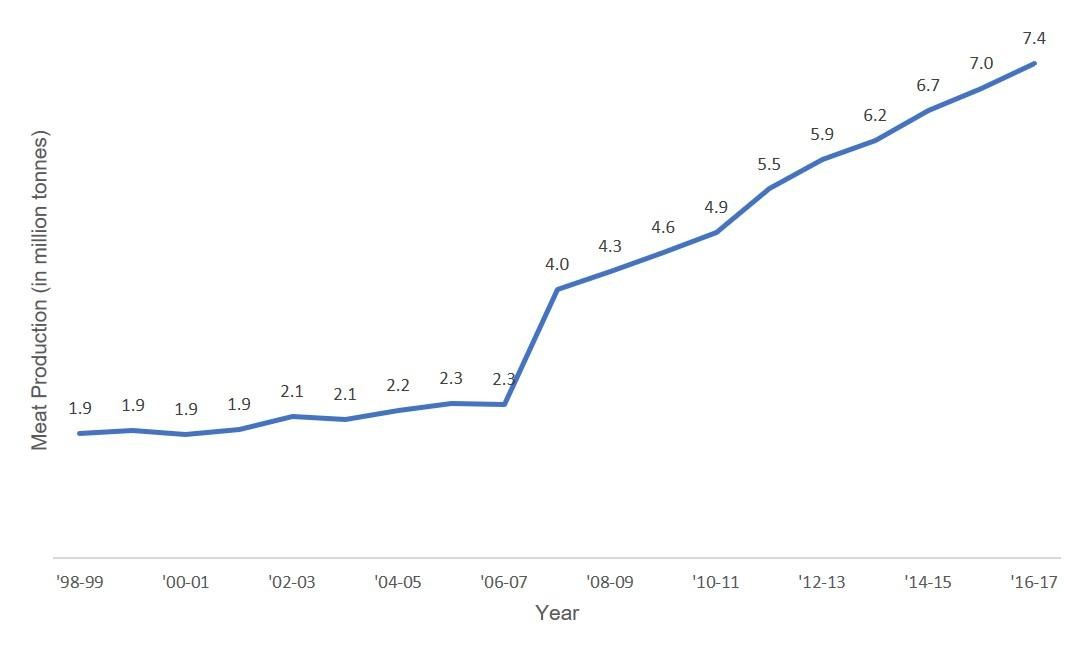
\includegraphics[height = 4.25in]{C:/Users/Dell/Desktop/CCS/TEX/New Folder/Fig 1.jpg}
%\caption[Optional Caption]{Figure 1: Total Meat Production in India From 1998-99 to 2016-17 \\ [\parencite{cmiestats}]}}
\end{figure}

However, the industry imposes significant negative externalities on the environment and is at the centre of emerging public health and hygiene concerns \parencite{praderepaper}. There are also several socio-cultural and religious constraints on the production and consumption of meat in India. All these, coupled with the need for ethical treatment of animals, attract government interventions in the sector. \\

Over the years, government has made ad hoc rules and amendments to existing regulations without adequate consultation, not harmonised conflicting objectives, and has attempted to pacify socio-cultural debate through instruments not fit for purpose. This has led to many unintended consequences.\\

First, sudden changes in the formulation and implementation of rules governing trade and property rights over animals have fomented business uncertainty. For example, the central Ministry of Shipping suddenly and indefinitely banned the export of livestock from ports in 2018 \parencite{kateshiyanews}. The ban was imposed just before the Bakr-Id festival when a large number of goats are exported to the Middle-East for religious sacrifices. News reports document that export of livestock, which had since 2013, witnessed a 56.06\% CAGR rise \footnote { The exports increased from Rs. 69.30 crore in 2013 to 2014 to Rs. 411.02 crore in 2017 to 2018.} in the value of export shipments, was suddenly stopped in its tracks and the ruling affected about 40,000 families \parencite{hindunews}. \\

Second, confusion created in law, coupled with the negative perception of meat traders and the already weak rule of law apparatus, has manifested in the form of vigilantism and violence. Several news reports have documented how traders are often attacked when transporting animals from farms to slaughterhouses. These cases and decisions have coalesced into a climate of fear among traders.\\

Third, incorrect public planning for slaughterhouses in cities such as Delhi constraints the supply chain of meat. This has led to the growth of unauthorised meat shops that also slaughter animals. The growth is, despite a clear restriction on the slaughter of any animal, within the premises of the shop. \\

Finally, the entry barriers to new businesses create difficulties in opening and operating formal businesses. The businessmen who do pay the one-time costs and obtain the licences are subjected to unclear and arbitrary inspections. These short- and long-term costs deter entrepreneurs from growing their business. \\

This paper examines the regulatory challenges with a focus on its impact on the small meat traders in Delhi. It describes the perceptions of various stakeholders and explores gaps between on-paper and on-ground policy. It also explores the licensing and inspections of slaughterhouses and meat shops—while scrutinizing the last two stages of the supply chain of meat in Delhi in greater detail.\\

There are four stages in the supply chain of meat. First, the rearing of animals on farms—the meat that is consumed in Delhi is mostly reared on farms in Haryana and Uttar Pradesh; second, the transportation and sale of these animals to a trader in a market or a murga mandi; third, the slaughter of these traded animals in a slaughterhouse; and fourth, the sale of meat that is extracted from the slaughtered animal in a meat shop. Figure 2 represents the supply chain of meat and the focus of our study. \\
Figure 2
\begin{figure}[H]
\centering
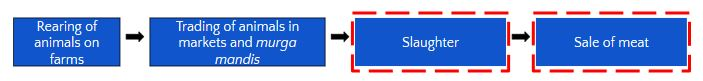
\includegraphics{C:/Users/Dell/Desktop/CCS/TEX/New Folder/Fig 2.jpg}
\caption[Optional Caption]{Figure 2: Supply Chain of Meat in Delhi}
\end{figure} 

The study of regulatory challenges with the slaughter of animals is based on secondary research and semi-structured interviews with individuals who are directly (business owners and exporters of livestock) or indirectly (journalists, lawyers and advocacy group members) involved in the meat industry of Delhi. We also interviewed officers of the relevant regulatory agencies such as the FSSAI and the Veterinary Department of the South Delhi Municipal Corporation (SDMC).\\

The study of meat shops was based on structured interviews of 52 shop owners to gauge their perception of licensing and inspection procedures. A mock inspection of 70 meat shops for 19 visually verifiable regulations was conducted to examine their compliance level. Further details of the methodology are in Appendix 1. 
\\

%Regulation of Slaughterhouses in Delhi
\section{Regulation of Slaughterhouses in Delhi}

A slaughterhouse or an abattoir is a facility where animals are slaughtered for consumption as food. The activities of slaughterhouses are sensitive for, broadly three reasons. First, the slaughter of an animal requires compliance with minimum hygiene and quality standards. Failure to maintain hygiene has a direct implication on public health. Second, slaughterhouse waste, constituting the inedible part of animals such as blood and other by-products, is polluting in nature and requires proper treatment and disposal. Third, arrangements to minimize animal suffering are required to preserve animal rights. This is done by ensuring adequate storage conditions, availability of food and water and compliance with a defined slaughter process alongside an inspection process.\\

The rules governing these issues are set by three central government agencies, the FSSAI, the Central Pollution Control Board (CPCB) and the Animal Welfare Board of India (AWBI). In Delhi state, our study geography, the Department of Food Safety, Government of National Capital Territory (NCT) of Delhi implements the regulations set by the FSSAI; the Delhi Pollution Control Committee (DPCC) implements the rules set by the CPCB; and the functions of the AWBI are performed by the MCD and the New Delhi Municipal Council.\\

\subsection{Prescriptive Requirements to Open and Operate a Slaughterhouse}

The regulating agencies use licences as the principal instrument to oversee and control the activities of slaughterhouses. While issuing licences, the corresponding agency specifies the requirements that each slaughterhouse needs to meet. It also conducts regular inspections to check their compliance during the course of operations. \\

Each regulatory agency issues its own licence. An entrepreneur must obtain the following licences in the given order to establish a slaughterhouse in Delhi:\\

\begin{enumerate}
\item Consent to Establish from the CPCB
\item No Objection Certificate (NOC) and a trade/storage licence from the MCD
\item Food Licence from the FSSAI
\item Consent to Operate from the CPCB.\\
\end{enumerate}

The imposed requirements, validity, processing time and fees for each licence vary. Details of the eligibility, time, cost are provided in Appendix 2, while the required documents are listed in Appendix 3. \\

\subsection{Barriers to Entry in Opening and Running a Slaughterhouse in Delhi}
The primary barriers on establishing a slaughterhouse are legal in nature. This consists of the licensing system and the statutory requirements laid out in acts and department regulations. They are described in the subsequent sections, which also examine their impact—both unintended and unintended.\\

\subsubsection{Prohibition on Operating Private Slaughterhouses in Delhi}

The MCD, one of the local governing bodies in the state of Delhi, is responsible for the planning of slaughterhouses and their operation. It was established through the Delhi Municipal Corporation (DMC) Act of 1957. \\

Section 42 of the DMC Act lists out the Obligatory Functions of the Corporation, stating, ‘[it] shall be incumbent on the Corporation to make adequate provision by any means or measures which it may lawfully use or take [on the matters listed in Section 42]. The regulation of slaughterhouses is included in Section 42 (k) making the MCD responsible, [for] the construction and maintenance of municipal markets and slaughterhouses and the regulation of all markets and slaughterhouses’.\\

The Act defines a slaughterhouse as ‘any place ordinarily used for the slaughter of animals for the purpose of selling the flesh thereof for human consumption’.\footnote{ As defined in S.2(56) of the DMC Act, 1957.}\footnote{ Permission for slaughter outside municipal slaughterhouses, albeit provided with the prior permission of the Commissioner, is restricted only for religious purposes.}, The two types of slaughterhouses are:\\

\begin{itemize}
\item Municipal slaughterhouses: ‘A slaughterhouse vested in or managed by the Corporation’ \footnote{ As defined in S.2(30) of the DMC Act, 1957.};
\item Private slaughterhouses: ‘A slaughterhouse which is not a municipal slaughterhouse’.\footnote{ As defined in S.2(41) of the DMC Act, 1957.}.\\
\end{itemize}

Despite defining a private slaughterhouse, the DMC Act in Section 407(2) states, ‘No place other than a municipal slaughterhouse shall be used as a slaughterhouse’\footnote{ Exceptions to this rule include the slaughter of any animal for any religious festival or ceremony in accordance to religious customs subject to the approval of the Commissioner, with the sanction of the Corporation.}. This effectively means that no animal can be slaughtered for consumption in any place except a slaughterhouse run by the MCD. As a result, no authorised privately owned slaughterhouses can be established and operated and a government monopoly is established over an essential service. \\

\subsubsection{Only Slaughterhouse in Delhi is Government-owned, Operated and Regulated}

The MCD owns and operates the only authorised slaughterhouse in Delhi. Located in Ghazipur, the MCD Ghazipur The slaughterhouse was opened in 2009 after sealing off a nearly 200-year old municipal slaughterhouse at Idgah near Jama Masjid. It was established to provide hygienic and modern facilities and expand production for export and local consumption. It has a capacity to process 5,000 small animals (goats and sheep) and 1,000 large animals (buffaloes) per shift \parencite{bhardwajnews}.\\

Currently, it is run on a public-private partnership model between the East Delhi Municipal Corporation and M/s Frigorifico Allanasons Pvt. Ltd. The operation is conducted in three shifts; morning and evening shifts are open for general traders, and the afternoon is reserved for the concessionaire—Frigorifico Allanasons.\\

\paragraph{Concerns with Conflicts of Interest}

The ownership status of the Ghazipur slaughterhouse does not exempt it from regulations; the FSSAI, MCD, AWBI and CPCB are still required to inspect and promote compliance with regulation. This is a conflict of interest and a departure from the doctrine of separation of powers. For instance, preventing cruelty to animals before and during slaughter is the responsibility of AWBI, the statutory body to advise the Government of India on laws aimed to prevent cruelty towards animals. But since the AWBI does not have its own enforcement mechanism, it executes its responsibilities through local governments. In Delhi, the responsibilities of AWBI are executed by the MCD.\footnote{ For example, the AWBI does not issue its own license to set up slaughterhouses. The requirements of AWBI are merged with the inspection checklist of the MCD for issuing the NOC.}\\

Under the existing incentive structure, it is often not in the interest of enforcement officials to penalize Ghazipur slaughterhouse for several violations which then remain unaddressed. A lack of independent oversight creates perverse incentives for the slaughterhouse to also hide faults from public view. \\

Reports and articles have highlighted several prima facie rule violations in the Ghazipur slaughterhouse. \\

\begin{itemize}
\item Food Safety and Standards (Licencing and Registration of Food Businesses) Regulations 2011 (FSSR 2011) \footnote{S.4.1 of Part IV of Schedule 4 of the FSSR 2011 states, ‘stunning before slaughter should be mandatory … [it] can avoid and minimise reactions of fear and anxiety as well as pain... among the animals concerned’.} and the PCA (Slaughter House) Rules 2001 \footnote{ S.6(4) of the PCA (Slaughter House) Rules, 2001 states, ‘Every slaughterhouse... shall provide a separate space for stunning of animals prior to slaughter, bleeding and dressing of the carcasses’.} both mandate the use of stunning before slaughter. They also require the use of a separate place for this process.
\item Buffaloes were electrocuted by placing a live wire on their body instead of being stunned \parencite{indiannews} \parencite{petareport}. However, the slaughter of animals through electrocution is rejected as a humane method for slaughter \parencite{chaudrypaper} and is in violation of Section A.6.(a) of the FSSR 2011.\footnote{ S.A.6(a) of Part IV of Schedule 4 of the FSSR 2011 states, ‘it is essential that animals be reared, handled, transported, and slaughtered using humane practices. A healthy and peaceful animal is an essential requirement for hygienic slaughter and safety of the meat product’.} Apart from being an act of cruelty against animals, electrocution also has an impact on the quality of meat obtained.
\item Animals were overcrowded in small lairages, that is, holding pens without adequate water and food \parencite{maanvinews}. This contradicts Section A.3.5 of Part IV of Schedule 4 of the FSSR 2011, which mandates the use of adequately sized lairages. \footnote{ S.A.3.5 of Part IV of Schedule 4 of the FSSR 2011 states, ‘the lairage shall be adequate in size for the number of animals to be laired’.}
\item Sick and pregnant animals were slaughtered without an ante-mortem examination (PETA 2009). This contradicts the Section 3 (2) of the PCA (Slaughter House) Rules, 2001, which states that any animal showing signs of disease should be condemned and rejected after an inspection. \footnote{ S.7(3) of Part IV of Schedule 4 of the FSSR 2011 states, ‘an animal showing signs of any disease at the time of ante-mortem inspection that would cause its carcass being ultimately condemned on post-mortem shall be marked as ‘condemned’ and rejected’.} The violation of this regulation is of particular concern as it directly impacts public health /parencite{mahaptranews}.

\end{itemize}

\paragraph{Concerns with Monopoly Market Power}

A state monopoly has several harmful consequences. Theorists have argued that a monopoly leads to an inefficient allocation of resources, management and production; output production below the market level; restrictions on the choice of consumers and a larger erosion of incentive for growth and amelioration in the absence of market competition and viable alternatives \parencite{mortonpaper}. \\

In the practical sense, this has three direct consequences.\\

\begin{enumerate}
\item Prohibiting the establishment of private slaughterhouses leads to a lack of alternatives and market competition. In the absence of viable alternatives, consumers are left with no choice on the products they purchase and consume. A consumer wanting to purchase meat produced in more hygienic conditions or with greater protection of animal rights has no options. Moreover, in the absence of any competition there is no incentive to bring about change or greater efficiency in the operation of the slaughterhouse. 
\item All meat traders in the state are dependent upon the supply from one slaughterhouse, which chokes the supply chain. 
\item The operations of this slaughterhouse are in part funded by taxpayer contributions who, regardless of their lifestyle choices, have to become a party to the slaughtering of animals. \\
\end{enumerate}

\subsubsection{All Chicken and Pig Slaughter in Delhi Is Officially Illegal}
The Ghazipur abattoir processes only buffalo, goat and sheep and has no provisions to slaughter chicken or pigs.\\ 

In Delhi, roughly 240,000 poultry birds are slaughtered every day to meet the daily demand while the daily pork consumption is about 120,000 kg, which requires the slaughter of around 2,000 pigs \parencite{singhnews}. Despite this sizeable demand, the regulations governing slaughter of meat in Delhi have rendered all forms of chicken and pig slaughter illegal, irrespective of any methods employed to prevent pollution and pain in the process. The regulations have created a deadlock for conducting business where traders of chicken cannot conduct business without circumventing the law.\\

Pig slaughter often takes place in swamps or wastelands adjacent to meat shops \parencite{tnnnews}. While the traders of pork have the option to avoid this by transporting processed meat from other states and selling it in Delhi, it leads to an increased cost. Leading meat retailers such as Khub Chand \& Bros. use this method of procuring meat.\\

While a pig abattoir in Rani Khera was conceived of in 2009 and is expected to be functional by 2021, Delhi neither has a legal slaughterhouse for chicken and pig, nor plans on making one for chicken. \\

Despite the fact that Section 407(2) of the DMC Act completely prohibits private slaughterhouses in Delhi and Section 9.05 of FSSR 2011 prohibits the slaughter of animals or birds inside the shop premises, chicken are slaughtered openly within the premises of meat shops.\footnote{According to S.9.05 of the FSSR 2011, ‘slaughtering of animal/birds inside the shop premises should be strictly prohibited’.} Buyers of chicken meat insist that it be freshly slaughtered, and transporting non-frozen chicken meat is not an option.

Recognising the catch-22, MCD inspectors allow meat shops selling chicken to slaughter them in the premises of their shop without the need of any additional licence by following an ‘unofficial policy’.\footnote{‘Additional’ here refers to the licenses that may be required over and above the ones required to establish a meat shop.} However, this policy apart, chicken shops are operating by breaking another law. \\

All 39 chicken shop owners we interviewed admitted to slaughtering chicken in their shops as a standard business practice. Despite this, 30 of these shops were either licensed by the MCD or registered with the FSSAI. Both, the FSSAI and the MCD have issued licences to several shops which clearly violate their regulations and do not fulfill the requirements to obtain the licences. This raises questions on the effectiveness of the licensing procedure in promoting compliance and vetting establishments which violate regulations. \\

The thoughtless regulatory set-up creates difficulties for businessmen who are vulnerable to rent seeking during inspections and the threat of penal action for violating the law. They also operate in a climate of uncertainty since the ‘unofficial policy’ has no written basis in law and can be revoked at any point of time. This also has a negative impact on consumers who, in the absence of an effective licensing and regulatory system cannot ascertain the quality of the meat they purchase. \\

Pork traders/retailers are also vulnerable to this regulatory dissonance. However, due to a separation between the shop and the area where pigs are slaughtered, it is only the slaughter of pig, and not its selling, which is under apparent scrutiny. This indicates the presence of a marginally better situation for the sale of pork in comparison to chicken which is most impacted by the inadvertent prohibition of private slaughterhouses. 

\section{Regulation of Meat Shops in Delhi}

After an animal is killed in a slaughterhouse, its meat is sold in shops, either whole or in smaller pieces. Such stores that sell meat are called meat shops. These include not only shops exclusively dealing in meat but also supermarkets and grocery stores that offer meat on their shelves.\\

The FSSAI and Department of Weights and Measures (DWM), alongside the MCD, are the regulatory agencies that oversee the activities of meat shops in Delhi. While the FSSAI and MCD regulate meat shops to ensure hygiene and quality of meat sold, the DWM ensures fairness and transparency in the scales employed for measurement of the meat sold. The DWM regulates only the sale of meat; the FSSAI and MCD regulate both the production at slaughterhouses and sale at meat shops. They distinguish, identify and define both parts of the supply chain, and have set out regulations and licences depending on whether the enterprise produces meat for consumption or sells it. \\

\subsection{Licenses Required to Open and Operate a Meat Shop}

The regulating agencies use licences as the principal instrument to oversee and control the activities of meat shops while upholding adequate standards of quality and hygiene. While issuing licences, the corresponding agency specifies the requirements that each meat shop needs to meet and conducts regular inspections to check their compliance during the course of operations. \\

To operate a meat shop in Delhi, the shopkeeper requires the following three licences:\\

\begin{enumerate}
\item Veterinary Licence from the MCD \footnote{ Unlike other retail establishments, meat shops come within the purview of the Veterinary and not Health Department due to the hygienic and environmental issues associated with meat.}
\item Food Licence from the FSSAI
\item Weights and Measurements certificate from the DWM.
\end{enumerate}

% Table generated by Excel2LaTeX from sheet 'Sheet1'
\begin{table}[htbp]
  \centering
  \caption{Add caption}
    \begin{tabular}{p{5.145em}p{7.855em}cccc}
    \textbf{Food Safety and Standards Authority of India, Department of Food Safety, Government of Delhi NCT} & \multicolumn{1}{r}{} &       &       &       &  \\
    The FSSAI regulates meat shops by laying down procedural requirements while listing tools and facilities each shop should have to ensure hygiene in storage and processing alongside quality control mechanisms. There are three categories within this, the details of which are listed below. & \multicolumn{1}{r}{} &       &       &       &  \\
    Central License & Turnover more than Rs. 20 crores & 7,500 & \multicolumn{1}{c}{\multirow{3}[0]{*}{Up to 5 years}} & 60    & 18 \\
    State License & Turnover between Rs. 12 lakhs and Rs. 20 crores & 2,000 &       & 60    & 18 \\
    Registration Certificate & Turnover up to Rs. 12 Lakhs & 100   &       & 7     & 7 \\
    \end{tabular}%
  \label{tab:addlabel}%
\end{table}%

Although licences are mandatory for businesses, they choose to remain unlicensed. Studies find that it is more cost-effective for them to stay unlicensed at their scale of operations because regulatory compliance would otherwise render them uneconomical \parencite{desotopaper} \parencite{duttapaper} \parencite{laportapaper}. In our survey of meat shops of Delhi, we witnessed similar claims and circumstances. Our findings are presented below. \\

\subsubsection{Licences Acquired by Respondents}
Of the 52 shops in the sample, 9 were completely unlicensed. Only three shops had all the necessary licences while the remaining had incomplete combinations.\\

Figure 3
\begin{figure}[H]
\centering
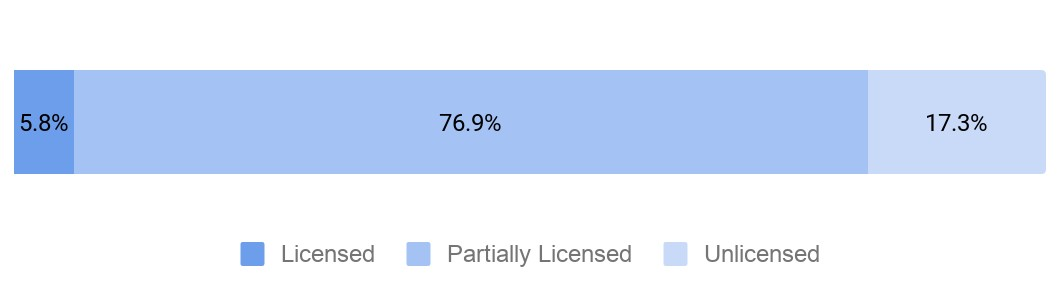
\includegraphics{C:/Users/Dell/Desktop/CCS/TEX/New Folder/Fig 3.jpg}
\caption[Optional Caption]{Figure 3: Percentage of Licensed, Partially Licensed and Unlicensed Respondents (n = 52)}
\end{figure} 

A majority of the licenced establishments only had a Veterinary licence. Numerous shop owners, when asked about the Food Licence, were unaware of it. Thus, despite being easier to obtain (see Figure 4), the Food Licence had not been obtained by 72.5\% of the respondents. The Weights and Measurements Certificate, which only requires the submission of one form, was also not obtained by 87\% of the respondents. \\

Survey respondents stated that the regulatory agencies conduct sealing drives to force unlicensed shops to acquire licence. For example, meat shop owners in the INA market acquired a Veterinary and Food Licence after the MCD and FSSAI sealed several shops in the vicinity in 2002 and 2012 respectively. An inspector in the Central Zone office of the SDMC also said that more than 100 unlicensed meat shops were closed in 2017.\footnote{ Refers to the Veterinary licence of the MCD.} In addition, FSSAI officers also claimed to conduct ‘extensive facilitation drives’ to improve the number of licence holders.\footnote{Claimed by a Designated Officer of the FSSAI Delhi State office. They also claimed their facilitation drives and registration centres to have enabled even the smallest meat shop owners to formalise.}
Despite this, 94.2\% of the respondents did not have all the requisite licences choosing to remain unlicensed or partially licenced.\\

The remaining unlicensed meat shops gave the following reasons for not obtaining the necessary licences:

\begin{itemize}
\item \textit{“Licensing can become unaffordable”}: Shopkeepers have to fulfill the necessary requirements listed by the MCD, FSSAI and DWM in order to acquire a licence. According to some shopkeepers, despite fulfilling these requirements, the official and unofficial cost of obtaining a licence can go up to Rs. 3-4 lakhs. Shopkeepers consider the cost of abiding by these regulations and acquiring licences to be prohibitively expensive and chose to keep their shops unlicenced.
\item \textit{“Operating from a Rented Premises”}: Most small shopkeepers rent their business premises. This creates complications in the licencing process as they are required to provide a permanent address or submit a greater number of documents for licensing the rented premise. 
\item \textit{“Too many documents required for obtaining a licence”}: A minimum of 23 documents must be submitted to obtain all the licences necessary to open a meat shop.\footnote{ See Table 2.} The availability of all these documents in proper order and condition was also considered as challenging by the shopkeepers.
\item \textit{“Difficulty in comprehending the regulations governing businesses”}: The regulations which span across three statute acts, four inspection checklists and several rules are often amended and written in complex legal jargon. When asked if regulations governing their business were easy to understand, 41 out of 52 shopkeepers responded as difficult.
\end{itemize}

\subsubsection{Ease of Obtaining Licenses}

All the licence required to run a meat shop formally cost between Rs. 600 and Rs. 12,000 (based on the turnover) and require between 60 and 120 days to process. As the cost and time indicated are contingent on providing adequate documents, the actual figures may vary. \\

To understand the perceived level of difficulty in acquiring these licence, we interviewed 33 licence holders (Figure 4).\\

Figure 4
\begin{figure}[H]
\centering
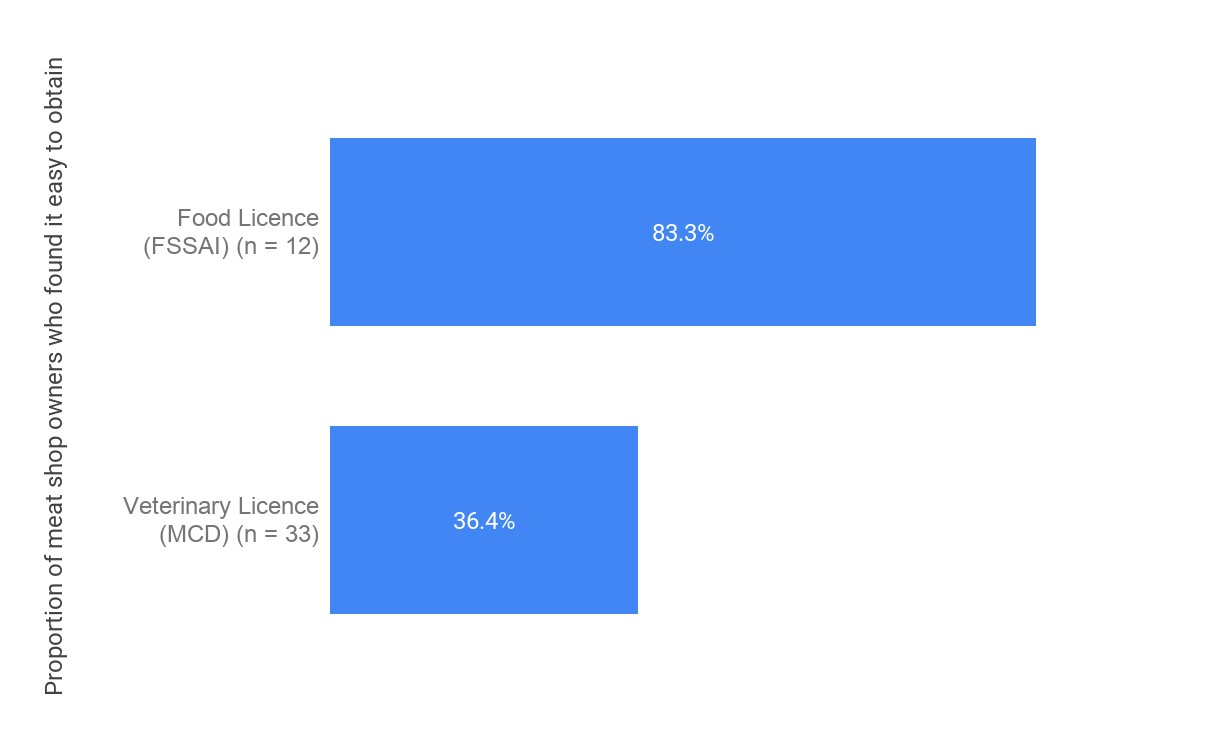
\includegraphics{C:/Users/Dell/Desktop/CCS/TEX/New Folder/Fig 4.jpg}
\caption[Optional Caption]{Figure 4: Perceived Level of Difficulty in Obtaining Licences\footnote{ The remaining respondents found it difficult to obtain these licences. We did not conduct a perception survey for the WMC because very few respondents had obtained it.}}
\end{figure} 

While the Veterinary Licence was seen to be more difficult to obtain than the Food Licence, a greater number of respondents chose to obtain it over the Food licence. \\

Due to difficulties in acquiring these licences, the shop owners resort to help from ‘third-party agents’ such as business consultants, touts and other influential people. Of the 43 people who were interviewed, about 25\% claimed to have received assistance from third-party agents. This is despite the digitization of the process and claims by both the MCD and the FSSAI to opening up several ‘facilitation centres’ to decrease the use of third-party agents and ease the process of obtaining licenses.\footnote{ As told to us by a Designated Officer in the FSSAI and an Inspector in the SDMC.} These centres were claimed to have been established in their administrative offices where officials could guide businessmen through the application process free of cost. \\

\subsubsection{Corruption in the Licensing Process}

Interaction with government officials while acquiring licences creates scope for corruption according to the respondents. To acquire the Veterinary Licence, about 72\% of the licence holders claimed to have paid more than the prescribed cost of Rs. 2,700 (Figure 5).\\

Figure 5
\begin{figure}[H]
\centering
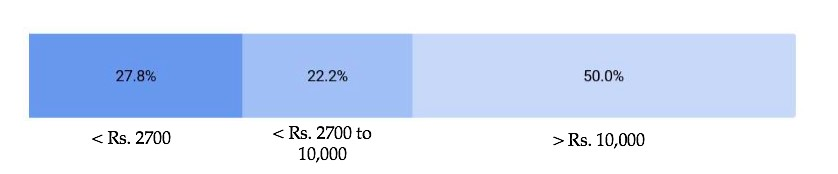
\includegraphics{C:/Users/Dell/Desktop/CCS/TEX/New Folder/Fig 5.jpg}
\caption[Optional Caption]{Figure 5: Amount in Rupees Paid to Obtain Veterinary Licence (n = 18)}
\end{figure} 

\subsection{Nature and Efficacy of the Inspections Regime Governing Meat Shops}

The MCD and FSSAI are the two agencies that inspect meat shops in Delhi. Their inspections are meant to ensure compliance with regulations, particularly those related to food quality and hygienic conditions (complete list of Inspection Requirements in Appendix 5). We investigated how both these agencies conduct inspections, and the efficacy of the inspection process in enforcing the rules. Based on interviews, surveys and mock inspections, we find that the existing inspection procedure is burdensome on meat shop owners who repeatedly cite it as a channel for rent seeking and disruption. The inspections are not only poorly managed and conducted but also ineffective in bringing about compliance. \\

\subsubsection{Distance of the Inspection Regime From Best Practices}

The Organisation for Economic Co-operation and Development (OECD), in their list of best practices and core principles which lead to effective enforcement, states that an inspection should follow an evidence-based enforcement, responsive regulation, transparent governance, clear and fair process alongside compliance promotion \parencite{oecd1report}. \\

We interviewed officials from inspectorates in Delhi and surveyed meat shop owners asking questions around each of these criteria to assess if the inspections regime that governs them is proportional, consistent and follows due process \parencite{oecd1report}. \\ 

\paragraph{Frequency}
The OECD best practices on risk focus and proportionality of the enforcement regime argue that, ‘the frequency of inspections and the resources employed should be proportional to the level of risk and enforcement actions should be aiming at reducing the actual risk posed by infractions’. \\

While the FSSR 2011 mandates at least an annual inspection of meat shops, the DMC Act only requires inspections to be ‘frequent’.\footnote{According to S.424 of the DMC Act and S.2.1.5(2) of Chapter 2 of Schedule 4 of FSSR 2011.} Neither specifies the criteria that qualify a business for inspections or their frequency. To ascertain the nature and frequency of inspections, we conducted interviews with inspectors from the South and Central Zone offices of the SDMC. Their responses were cross-verified with the meat shops in their corresponding region. \\

Inspectors from the SDMC claimed to inspect every establishment once a year. However, the responses from the surveys indicate a frequency of at least once a month, 12 times higher a number than that reported by inspectors. The distribution of monthly inspections is represented in Figure 6. \\

Figure 6
\begin{figure}[H]
\centering
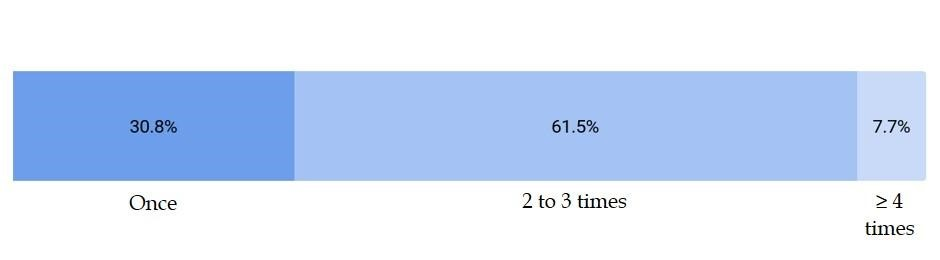
\includegraphics{C:/Users/Dell/Desktop/CCS/TEX/New Folder/Fig 6.jpg}
\caption[Optional Caption]{Figure 6: Claimed Frequency of Inspections Per Month (n = 52)}
\end{figure} 

\paragraph{Transparency}

Transparency relates to the public availability of information on the inspections process to be followed and expectations from business owners \parencite{blancreport}. Transparency of inspections can be facilitated through the use of an \textit {inspection checklist} which lays down the parameters on which a business is to be judged during inspections and controls the excesses of the inspectors. The OECD best practices for a transparent process state, ‘coherent legislation to organise inspections and enforcement needs to be adopted and published, and clearly articulate rights and obligations of officials and of businesses’ \parencite{oecd1report}.\\

While the FSSAI has a published inspection checklist on their website and office, the checklist of SDMC is neither officially published nor publicly available \footnote{ The SDMC inspection checklist was obtained from a Veterinary Inspector on the condition of anonymity.}(see Appendix 6). \\

During interviews, inspectors from both the SDMC and the FSSAI mentioned that checklists are used during inspections. However, about 81\% of meat shop owners (out of 43) were unaware of the parameters that were inspected, which makes it difficult for the shopkeepers to comply with them. \\

\paragraph{Procedural Fairness}

Procedural fairness relates to the following processes that are both fair to the rights of the businesses and clear on the limitations of the inspectors \parencite{oecdreport}. The two key elements that facilitate procedural fairness of inspections are inspection reports and process of prosecution on non-compliance.\\

\subparagraph{Inspection Report}

It is a document that establishes a detailed record of events (date, time, duration, inspecting officer, compliance level, violations, evidence of violations etc.) from the inspection visit. These reports act as the proof of inspection, ensure coherency between observation and reporting and hold both the parties accountable (businessmen for violations and inspectors for corrective measures). \\

A Veterinary Inspector from the Central Zone of the SDMC claimed to record his findings on the inspection checklist that also doubles up as an inspection report.\footnote{The inspection checklist is mandated to be carried during inspections. It also contains a provision to record the findings.} A Designated Officer from the Delhi state office of the FSSAI described a similar system to us.\\

Figure 7
\begin{figure}[H]
\centering
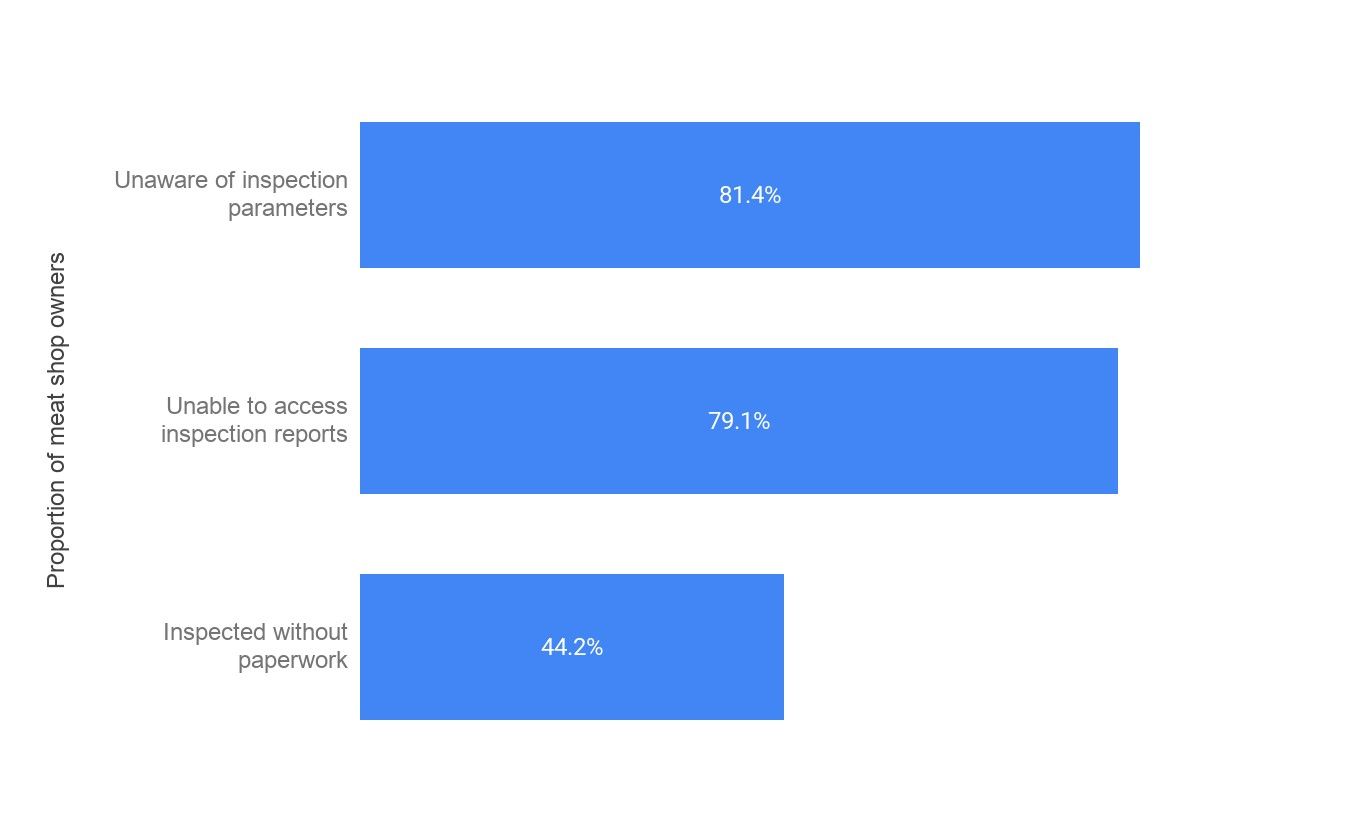
\includegraphics{C:/Users/Dell/Desktop/CCS/TEX/New Folder/Fig 7.jpg}
\caption[Optional Caption]{Figure 7: Lack of Awareness of Transparency and Procedural Fairness Parameters \footnote{ These were binary response questions. The remaining respondents said yes.} (n = 43)}
\end{figure} 

The claims of the officers, however, were not supported by the survey respondents (see Figure 7); 44\% of the survey respondents said that inspectors often maintained neither paperwork nor records of the inspections. Moreover, 81\% (35 out of 43) of the respondents reported being unable to view or access the inspection reports. This meant that the businesses did not know their alleged violations and had no access to their case files. Of the respondents who accessed the report, about 55\% (five of the nine respondents) were unable to appeal against the report. \\

A key function of these reports while ensuring transparency is also to promote compliance among shop owners. Lack of access to inspection reports impedes the meat shop owners’ ability to address faults and improve compliance. This also affects the process of appeal, restricting a shop owner’s ability to challenge inaccurate or false inspection reports.\\

\subparagraph{Prosecution on Non-compliance}

Section 68 of The Food Safety \& Standards Act, 2006, lays down the process of adjudicating a case of non-compliance. It states that ‘an officer not below the rank of Additional District Magistrate of the district where the alleged offence is committed, shall be notified by the State Government as the Adjudicating Officer… The Adjudicating Officer shall, after giving the person a reasonable opportunity for making representation in the matter’. The Adjudicating Officer can impose such penalty as he thinks fit based on provisions relating to the offence. Offences include selling substandard food or food not of the nature of quality demanded, failure to comply with regulations and directions of Food Safety Officers (FSOs), obstructing an FSO from exercising his functions, carrying out a business without a licence, etc. Each violation has a defined punishment.\\

The ability of the FSSAI to monitor and enforce compliance in Delhi is severely constrained by a shortage of inspectors. The FSSAI currently has only 25 Food Inspectors tasked with inspecting all Food Business Operators (FBOs) in Delhi.\\

The DMC Act, however, does not specify any such process in the case of non-compliance. However, the MCD inspectors claimed that a procedure for prosecution does exist. During interviews, they outlined a three-step process that is followed in the case of non-compliance:\\

\begin{itemize}
\item \textit{Improvement notice}: On observing a violation during inspections, an improvement notice is served to the establishments. It specifies the violated regulations and provides a period of 15 days to make amends and ensure compliance.
\item \textit{Challan or a show cause notice}: If not complied with despite the improvement notice, a challan or a show cause notice is served. While the challan is a fine paid by the licenced establishments for repeated non-compliance, a show cause notice requires the meat shop to justify against any action towards him. It is served before the closure notice and given 15 days to reply. 
\item \textit{Closure notice}: If not complied with despite the challan and show cause notice, a closure notice is served. Once served, the shop can be closed with immediate effect. These closure notices are also used as a deterrent tool against unlicenced establishments that consistently violate regulations. 
\end{itemize}

However, the choice between these deterrence tools is left to the inspector. While it is necessary to serve a show cause notice before a closure notice, it is up to the discretion of the inspector to serve a \textit{challan}. This discretion leads to arbitrary powers to impose punishments. \parencite{roychapter} capture the consequences of arbitrary power with inspectors in awarding punishment: ‘This leads to arrogance and corruption. If investigators and prosecutors know they can easily inflict punishment, they lose the incentive to do thorough work’.\\

The three-step process does not apply to unlicensed \footnote{ Refers to the Veterinary License of MCD.} meat shops. The MCD has the power to directly issue a closure notice to these shops.\\

Figure 8
\begin{figure}[H]
\centering
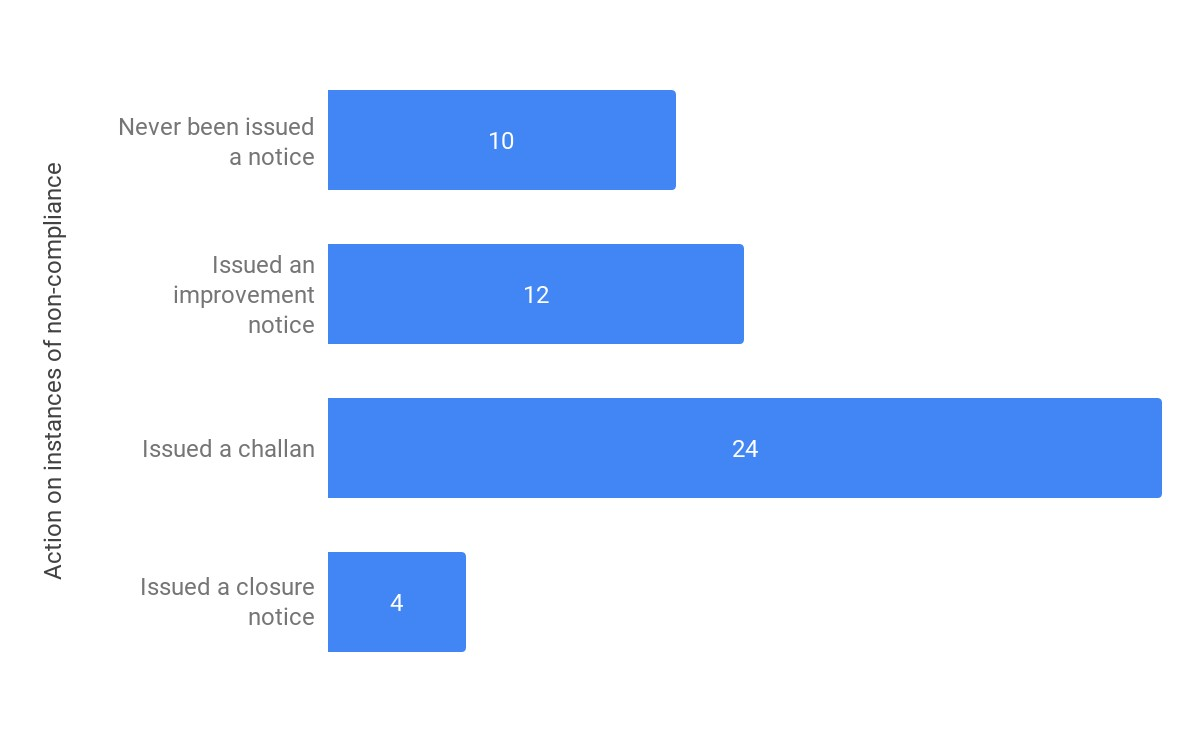
\includegraphics{C:/Users/Dell/Desktop/CCS/TEX/New Folder/Fig 8.jpg}
\caption[Optional Caption]{Figure 8: Notices Issued to Licenced Meat Shops (n = 43) \footnote{None of the respondents in our sample were given a show cause notice instead of a \textit{challan}.}}
\end{figure}

While inspectors from the SDMC state that a challan is given only on repeated non-compliance and after improvement notices, our survey results contradict the claim. Responses in Figure 8 show that among licenced shops, the number of challan recipients is greater than that of improvement notices. Meat shop owners say that the challan amount ranges from Rs. 100 to Rs. 3,000.\footnote{However, according to a meat shop owner in Jamia Nagar, the challan amount was increased from Rs. 500 to Rs. 2000 in 2016 without any prior information.} When asked about whether it was clear as to what would happen in the case of non-compliance, nearly 90\% of respondents were unaware of the specified penalties for the violations. We searched public fora to find penalty specifications but came up empty.\\

\subsubsection{Efficacy of Inspections in Promoting Compliance}

The objective of meat shop inspections is to ensure their compliance with regulations, which are aimed at mitigating negative externalities on the environment and public health and hygiene concerns. Interviews with meat shop owners indicate that inspections occur frequently. Moreover, MCD inspections seem to be occurring at least once a month. Now while this is prima facie evidence that inspections are at least being conducted, it does not provide any insight on whether the inspections meet their objective. We inspected 70 meat shops to assess levels of compliance on 19 regulations (from the inspection checklists of the MCD and FSSAI)./footnote{For complete checklists, see Appendix 6.} These regulations were deliberately chosen for being easily verifiable through mere visual inspections. We found that only 2 of the 70 shops in the sample complied with more than 80\% of the rules we checked for, indicating widespread non-compliance with rules despite frequent inspections conducted. 

The findings from our inspection are presented in Table 2. \\

%TABLE

While the primary purpose was to observe the efficacy of the inspection process, substantive concerns on the responsiveness of regulation also emerged. For example, checklists specify regulations meat shop owners saw as incompatible with prevalent business practices and customer needs. \\

\section{Conclusion}

This paper examined the regulatory framework binding slaughterhouses and meat shops in Delhi. We scrutinized the prescriptive requirements to open and operate slaughterhouses and a meat shop. We also conducted a perception survey with meat shop owners for the licences required and inspections conducted to regulate meat shops.\\ 

First, regulations such as the ban on all private slaughterhouses are often drawn without considering their indirect consequences. This negligence leads to the prevalence of informality and a government monopoly over the slaughter of animals. It creates a concentration of supply and lack of market competition and alternatives. The MCD also lacks a separation of powers between its role as a regulator and a service provider, giving rise to non-compliance.\\

The absence of any legal slaughterhouses for chicken and pork leads to concerns over public health, product quality and soil and water contamination. Moreover, in the current framework, every single shop slaughtering birds or animals is illegal irrespective of hygiene followed or methods employed. Unauthorised slaughterhouses including facilities at Khanpur, Mehrauli and Said Ul Ajaib operate to meet the gap between the demand of the city and the supply of the Ghazipur slaughterhouse. Owing to the regulations which make their operation illegal, these slaughterhouses are forced to operate stealthily, lest they attract government supervision. \\

Second, of the three licences required to open and operate a meat shop, the Veterinary Licence and Food Licence are overlapping in their requirements and inspection parameters. Given the wide range of requirements, it is difficult to see how and why even well-meaning entrepreneurs could comply. We find that a vast number of meat shop owners are choosing to stay unlicenced. This indicates a possibility where the operational costs while complying with regulations are higher than the benefits. It also suggests that the regulations prescribed are not high on the list of consumer criteria for purchase. Under the circumstances, it is not hard to imagine a scenario of pervasive rent seeking and an inability to collateralise assets and grow using formal credit. \\

Third, despite a high frequency of inspections conducted, non-compliance of regulations among licenced establishments is prevalent. This indicates that inspections are often ineffective in promoting compliance and can also digresse into channels of rent seeking. Lack of public availability of MCD inspection checklists, access to inspection reports for increased transparency and procedural fairness also need to be tackled. The distance between the existing inspection practices and the OECD best practices indicates a need to rethink and redraw both the licensing and inspections rules to close this gap. There is a need to review both the FSSAI and MCD regulations while keeping in mind their intended application and context applicability and also setting limits to the arbitrary powers of inspectors. \\

% Print Bibliography

\printbibliography[title={Bibliography}]
%Appendix1
\newpage 
\section*{Appendix 1: Methodology}
\addcontentsline{toc}{section}{Appendix 1: Methodology}
The findings in the paper are based on semi-structured interviews with individuals who are directly (business owners and exporters of livestock) or indirectly (journalists, lawyers and members of advocacy groups) involved in the meat industry in Delhi alongside officers from relevant regulatory authorities. A list of the interviewees and their relevance to the industry are provided in Table 3. 
%TABLE
All the shops were sampled from the major meat markets of South and Central Zones of SDMC. The interviewees were selected from carabeef (buffalo meat), chicken and mutton sellers. A description of the sample that was interviewed is provided in Table 4.

%Appendix2
\newpage
\section*{Appendix 2: List of Licenses Required to Set Up a Municipal Slaughterhouse}
\addcontentsline{toc}{section}{Appendix 2: List of Licenses Required to Set Up a Municipal Slaughterhouse}
%TABLE
%Appendix3
\newpage
\section*{Appendix 3: Documents Required for Licenses for Slaughterhouses}
\addcontentsline{toc}{section}{Appendix 3: Documents Required for Licenses for Slaughterhouses}
%TABLE

%Appendix4
\newpage
\section*{Appendix 4: Questionnaire for Meat Shop Owners}
\addcontentsline{toc}{section}{Appendix 4: Questionnaire for Meat Shop Owners}
\setstretch{0.5}
\begin{mdframed}[backgroundcolor=gray!20]
\textbf {Section 1}
\begin{enumerate}[noitemsep]
\item What products do you sell?
\item Where do you source your meat from?
\end{enumerate}
\textbf {Section 2}
\begin{enumerate}[noitemsep]
\item What licences do you have?
\item When did you take these licences?
\item Was it easy or difficult to obtain a licence from the MCD? (Easy/Difficult)
\item Was it easy or difficult to obtain a licence from the FSSAI? (Easy/Difficult)
\item How much did it cost (formally and informally) to obtain a Veterinary Licence?
\item Did you hire any third-party agency for the licencing process? (Yes/No)
\item How often do you receive the MCD and FSSAI licences renewed?
\item If you are unlicensed, why?
\end{enumerate}
\textbf {Section 3}
\begin{enumerate}[noitemsep]
\item How many times per month do government officials visit your shop for inspections?
\item Are you aware of what government officials look for when they come for inspections? (Yes/No)
\item Which of the following government notices have you been issued? (Improvement Notice/Show Cause Notice (\textit{Challan})/Closure Notice/No, I have never been given a notice)
\item Is it clear as to what would happen if you were found to be non-compliant with the regulations? (Yes/No)
\item Are post-inspection reports available to you? If yes, can you challenge them? (Available and can challenge/Available but cannot challenge/Not available)
\item Are all inspections conducted formally with paperwork filed? (Yes/No)
\end{enumerate}
\textbf {Section 4}
\begin{enumerate}[noitemsep]
\item Are the regulations governing your business easy to understand? (Yes/No)
\item Is the administration open to questions on regulations asked by you? If yes, do they give precise answers? (Yes, and give precise answers/Yes, but don’t give precise answers/No)
\item Do you have multiple people to contact within the administration? If yes, do they all give the same answers? (Yes, and they give same answers/Yes, but they don’t give same 
answers/No)
\end{enumerate} 
\end{mdframed}

%Appendix5
\newpage
\section*{Appendix 5: Documents Required for Licenses for Meat Shops}
\addcontentsline{toc}{section}{Appendix 3: Documents Required for Licenses for Meat Shops}
%TABLE

%Appendix6
\newpage
\section*{Appendix 6: Inspection Requirements for Meat Shops}
\addcontentsline{toc}{section}{Appendix 6: Inspection Requirements for Meat Shops}
%TABLE
\end{document}
\bibliography{meat}{}
\bibliographystyle{plain}
